\documentclass[12pt]{article}
	
\usepackage[margin=1in]{geometry}		% For setting margins
\usepackage{amsmath}				% For Math
\usepackage{fancyhdr}				% For fancy header/footer
\usepackage{graphicx}				% For including figure/image
\usepackage{cancel}				% To use the slash to cancel out stuff in work
\usepackage[spanish]{babel}
\usepackage{hyperref}
\usepackage{enumitem}
\usepackage{float}
\usepackage[utf8]{inputenc}


\pagestyle{fancy}
\fancyhead[LO,L]{Base de Datos}
\fancyhead[CO,C]{SIA 301 - Almacenar Paswords}
\fancyhead[RO,R]{14 de noviembre de 2023}
\fancyfoot[LO,L]{}
\fancyfoot[CO,C]{\thepage}
\fancyfoot[RO,R]{}
\renewcommand{\headrulewidth}{0.4pt}
\renewcommand{\footrulewidth}{0.4pt}

\begin{document}
\noindent \textbf{Universidad Nacional del Altiplano\\
Docente: } Fred Torres Cruz\\
\textbf{Estudiante:} Ronald Alex Diaz Pari

\vspace{2mm}
\noindent\textbf{Trabajo Encargado N°6}\\
\section{Registro de usuarios}

\begin{figure}[H]
    \centering
    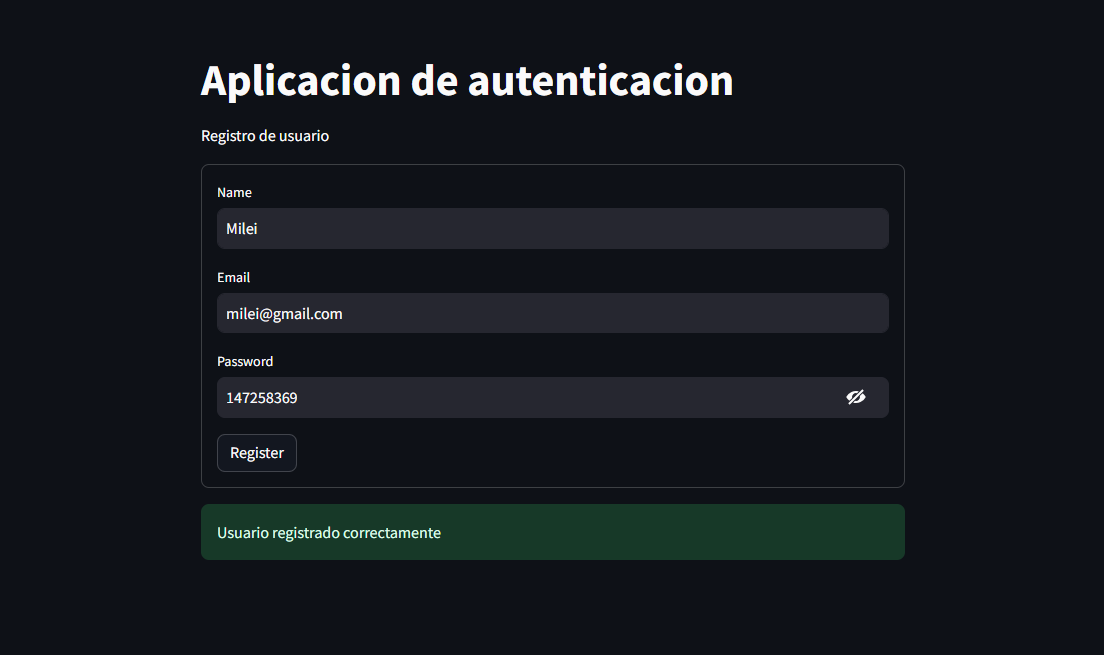
\includegraphics[width=1\textwidth]{./img/Register.png}
    \caption{ventana de registro de usuarios}
    \label{fig:my_label}
\end{figure}


\section{Ventana de login de usuarios}
\begin{figure}[H]
    \centering
    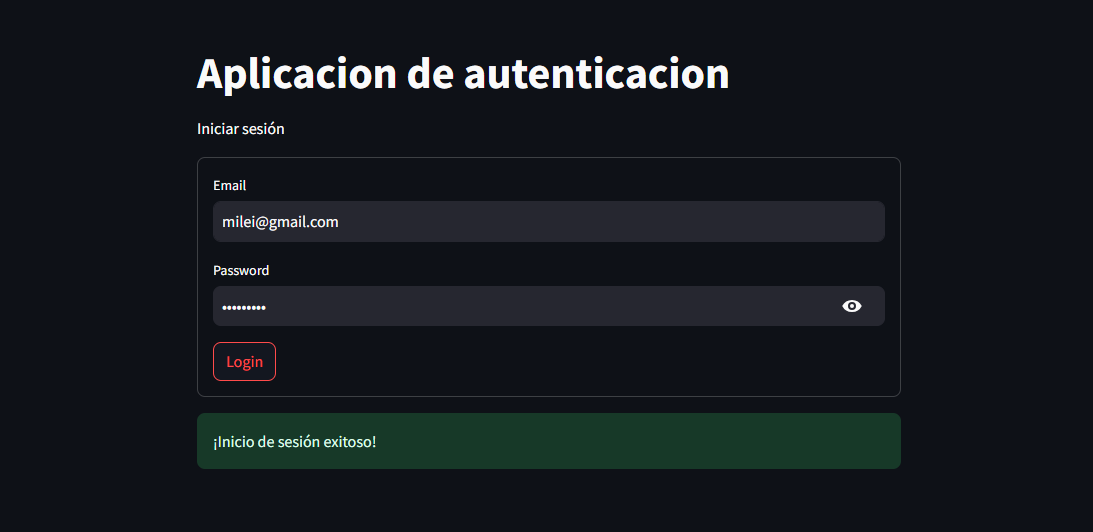
\includegraphics[width=1\textwidth]{./img/Login.png}
    \caption{Ejemplo de uso del login de usuarios}
    \label{fig:my_label}
\end{figure}


\section{Base de datos en MYSQL}
\begin{figure}[H]
    \centering
    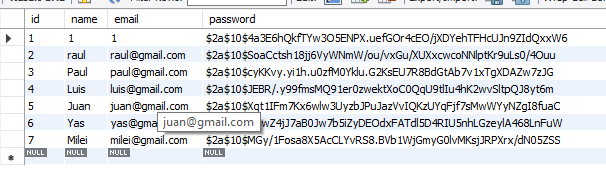
\includegraphics[width=1\textwidth]{./img/DB-Mysql.png}
    \caption{Foto de la tabla users en la base de datos app}
    \label{fig:my_label}
\end{figure}
\section{Sentencias SQL para crear la base de datos y la tabla de usuarios en MYSQL}

\large{Crear base de datos de la aplicacion}
\begin{verbatim}
    CREATE DATABASE app_auth;
    use app_auth;
\end{verbatim}

\large{Crear tabla de users en la base de datos app}

\begin{verbatim}
    CREATE TABLE IF NOT EXISTS users(
        id INT AUTO_INCREMENT PRIMARY KEY NOT NULL,
        name VARCHAR(255) NOT NULL,
        email VARCHAR(255) UNIQUE NOT NULL,
        password VARCHAR(255) NOT NULL,
    );

\end{verbatim}
\large{Insertar un usuario en la tabla users}
\begin{verbatim}
    INSERT INTO app_auth.users(name, email, password)
    VALUES('milei', 'milei@gmail.com', '$2a$10$MGy/');
\end{verbatim}

\section{Cifrado de contraseñas usando bcrypt y argon2}

\large{Cifrado de contraseñas usando bcrypt}
\begin{verbatim} 
    def hash_password_bcrypt(password):
        salt = bcrypt.gensalt(
            rounds=10,
            prefix=b'2a'
        )
        hashed_password = bcrypt.hashpw(password.encode('utf-8'), salt)
\end{verbatim}

\large{Cifrado de contraseñas usando argon2}
\begin{verbatim} 
    def hash_password_argon2(password):
        ph = PasswordHasher()
        hashed_password = ph.hash(password)
        return hashed_password
\end{verbatim}

\section{Codigo fuente de la aplicacion}

% link
\large \textbf{Link:}
\url{https://github.com/}


\end{document}
